\subsection{\large{\textit{tP}12-SiO\textsubscript{2} (Direct)}}\vspace{-0.1in}
Cristobalite ($\alpha$, HT)


\begin{figure}[H]
\begin{minipage}{0.34\textwidth}\centering
\includegraphics[width=0.9\linewidth,height=2in,keepaspectratio]{/Users/rosecers/work_folders/structures_for_photonics/reference/ref_inp/workspace/3f1324b110f31bd22dbe9d9d4cb078c9/final_images/analog_trim.jpg}\\
\small{Image of \textit{tP}12-SiO\textsubscript{2}, generated by Vesta}
\end{minipage}\hfill
\begin{minipage}{0.65\textwidth}\raggedright
{\setlength{\mathindent}{0cm}
\begin{equation*}
\begin{split}&\boldsymbol{a_1} = \ \hat{x}\\[-8pt]
&\boldsymbol{a_2} = \ \hat{y}\\[-8pt]
&\boldsymbol{a_3} = 1.3977078859161431\ \hat{z}
\end{split}
\end{equation*}}

\textbf{Space Group:}	92\hspace{0.5in}\textbf{Point Group:}	$422$\\
\textbf{Inorganic Crystallographic Database} \#34928\\
\textbf{Structure DOI: }\url{10.1524/zkri.1973.138.jg.274}

\end{minipage}\hfill
\end{figure}
\vspace{-0.25in}


\begin{figure}[H]
\begin{minipage}{0.9\textwidth}\centering
\includegraphics[width=0.9\linewidth,height=2.5in,keepaspectratio]{/Users/rosecers/work_folders/structures_for_photonics/reference/ref_inp/workspace/3f1324b110f31bd22dbe9d9d4cb078c9/final_images/gap_atlas.jpg}
\\
\end{minipage}\hfill\caption{Gap Atlas across filling fraction $\phi$ and frequency $\omega$}
\end{figure}


\begin{figure}[H]
\begin{minipage}{0.5\textwidth}\centering
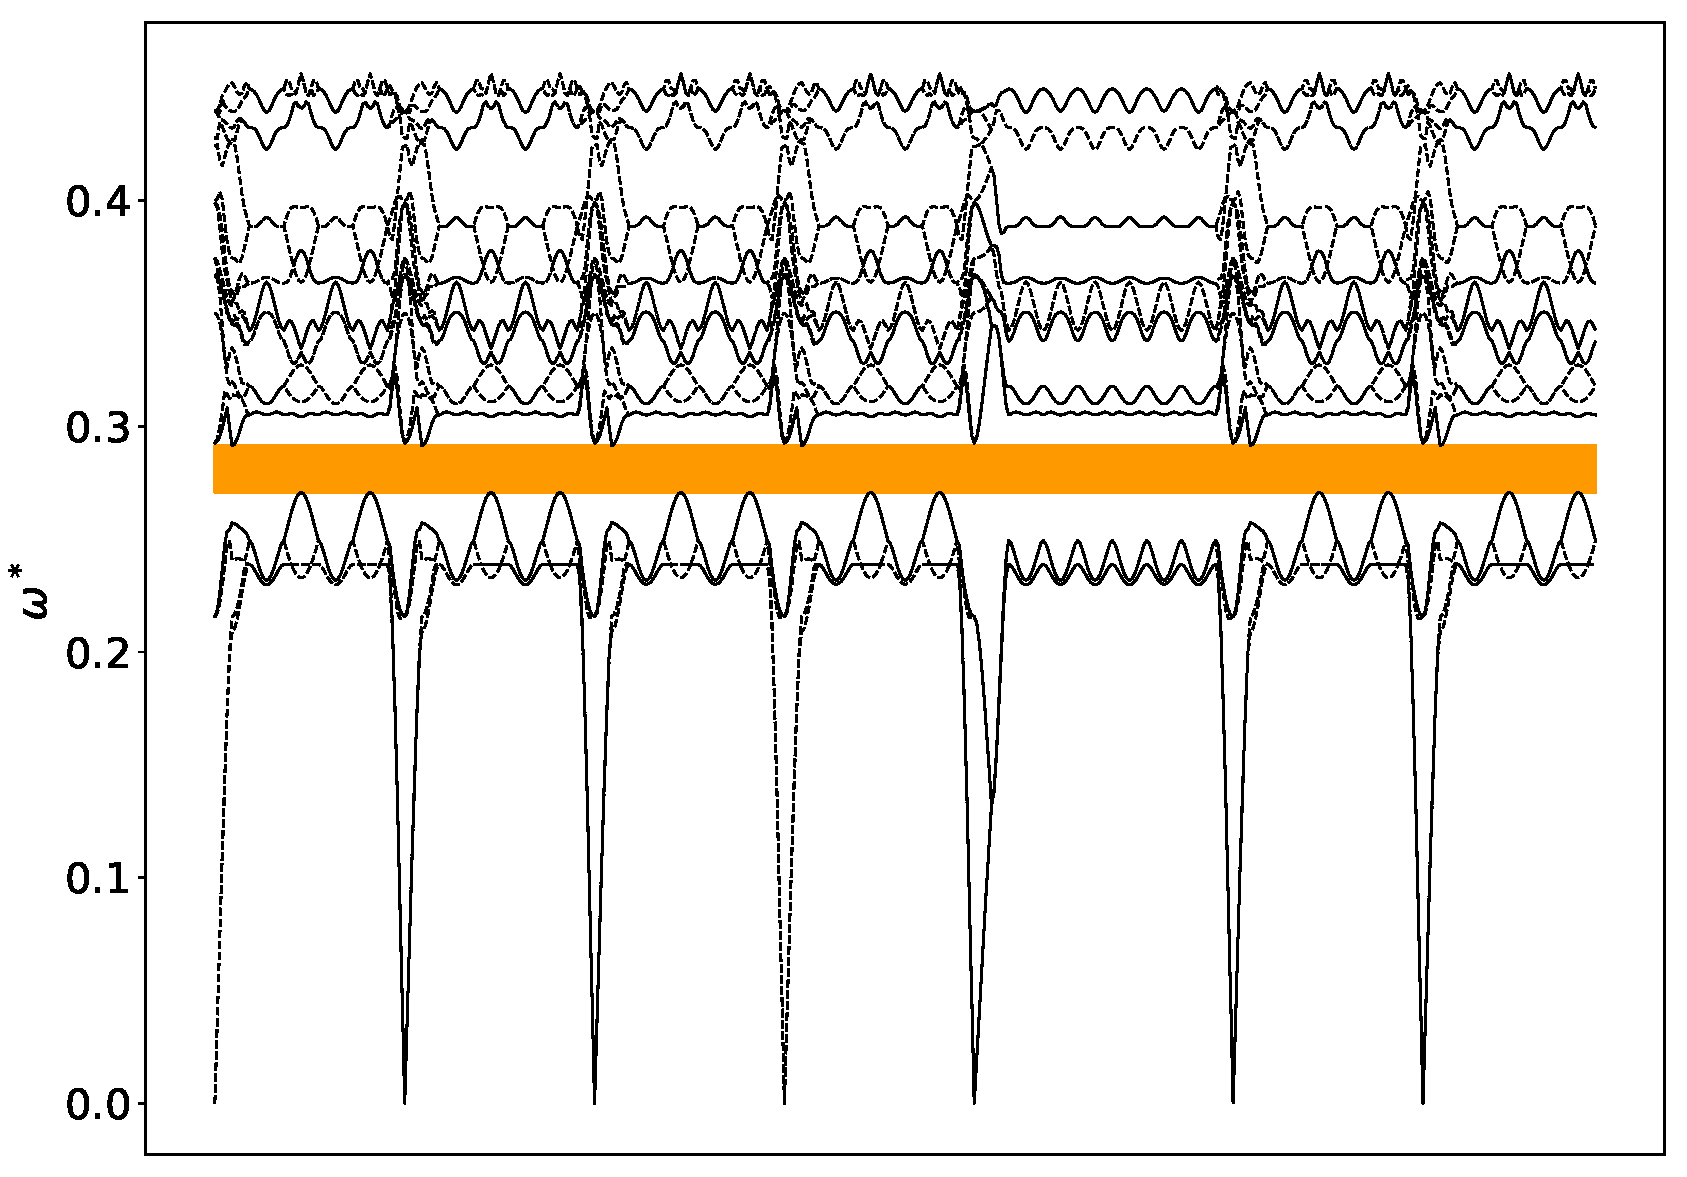
\includegraphics[width=0.9\linewidth,height=1.5in,keepaspectratio]{/Users/rosecers/work_folders/structures_for_photonics/reference/ref_inp/workspace/3f1324b110f31bd22dbe9d9d4cb078c9/./final_images/band_diagram_b=4.pdf}
\\Band Structure across 1st BZ
\end{minipage}\hfill
\begin{minipage}{0.28\textwidth}\centering
\includegraphics[width=0.9\linewidth,height=1.5in,keepaspectratio]{/Users/rosecers/work_folders/structures_for_photonics/reference/ref_inp/workspace/3f1324b110f31bd22dbe9d9d4cb078c9/final_images/tP12-SiO2@gap_4-5.png}
\\View along $a_2$ 
\end{minipage}\hfill
\begin{minipage}{0.2\textwidth}\centering
\includegraphics[width=0.9\linewidth,height=1.5in,keepaspectratio]{/Users/rosecers/work_folders/structures_for_photonics/reference/ref_inp/workspace/3f1324b110f31bd22dbe9d9d4cb078c9/final_images/tP12-SiO2@gap_4-5_1.png}
\\View along $a_1$ 
\end{minipage}\hfill\caption{Band Structure and Isosurface of \textit{tP}12-SiO\textsubscript{2} (Direct) at radius = 0.2, filling fraction = 0.036, where the largest gap between bands 4 and 5 occurs with gap size 24.44\%.}

\end{figure}
\vspace{-0.25in}

